\vspace{-5pt}
\section{Novel-View Synthesis}
Once the scene has been trained as per the previous chapter, we can use the camera matrices of a novel view and execute the existing forward pass to render a new image.

\vspace{-5pt}
\section{Conclusion \& Outlook}
Kerbl et al. did not invent 3D Gaussians, nor splatting, nor 3D covariance matrix decomposition, nor spherical harmonics, nor neural or differential rendering, nor alpha compositing, nor explicit radiance fields, nor many other technologies. They experienced the progress and the remaining limitations that NeRFs brought yet whitnessed even explicit radiance field solutions for NeRFs not reaching real-time novel-view synthesis.

However, they resurrected 3D Gaussian Splatting from the depths of academia and repurposed it for the current age, took all of these existing components and experiences and realized that decomposing a 3D covariance matrix into scale and quaternions would always yield a geometrically valid covariance matrix and that passing these two components separately into backpropagation would elegantly solve previous issues.

The other half of what they contributed with 3DGS was how elegantly their algorithm fit onto the hardware, especially the ultra-fast Radix Sort and tile-based rasterizer.

3DGS has made easy 3D reconstruction feasible leading to many adaptions in real-world scenarios and ongoing massive research in the field, e.g. exceeding \textit{1000} FPS in special types of novel-view synthesis \cite{NEURIPS2025_6c39d1a7} or advances in SLAM in robotics \cite{keethaSplaTAMSplatTrack2024}, and many more.
\newpage

\appendix

\section{Figures}

\begin{figure}[H]
    \centering
    \begin{subfigure}{0.45\textwidth}
        \centering
        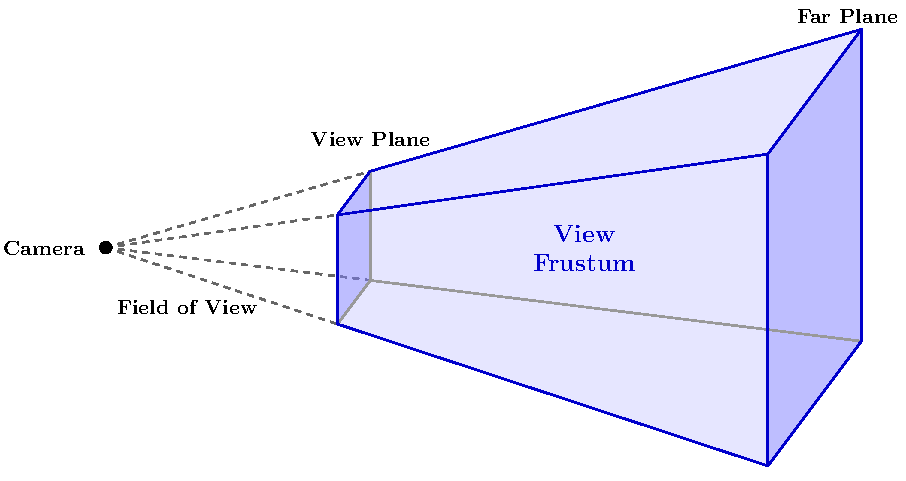
\includegraphics[width=\textwidth]{figures/view_frustum.pdf}
        \caption{View Frustum}
        \label{fig:view_frustum}
    \end{subfigure}
    \hfill
    \begin{subfigure}{0.45\textwidth}
        \centering
        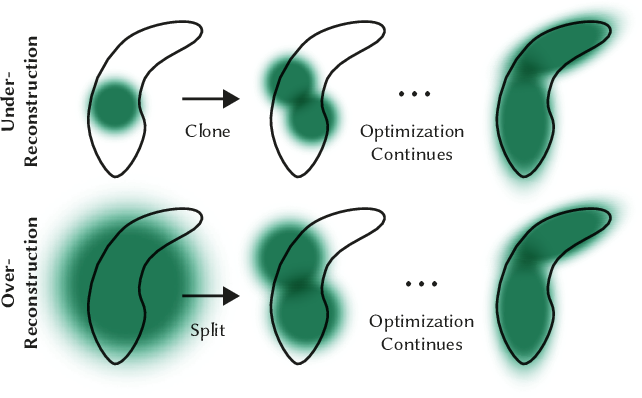
\includegraphics[scale=0.26]{figures/6-Figure4-1.png}
        \caption{Adaptive Density Control (from \cite{kerbl3DGaussianSplatting2023})}
        \label{fig:adc}
    \end{subfigure}
\end{figure}